\documentclass{ximera}

\title[Examples:]{Intro goniometrie}

\begin{document}
\begin{abstract}
	Hoeken (en dus driehoeken, cosinussen, ...)
\end{abstract}
\maketitle


Goniometrie (of driehoeksmeetkunde) is de studie van hoeken, en wordt gebruikt in tal van wetenschappelijke disciplines. Landmeters gebruiken bijvoorbeeld een theodoliet om hoeken te meten, en op basis daarvan afstanden te berekenen. De krachten in complexe staalconstructies  kunnen dikwijls berekend worden op basis van driehoeken. In een elektriciteitsmast kan je de driehoeken gewoon zien!

\begin{center}
\begin{image}
	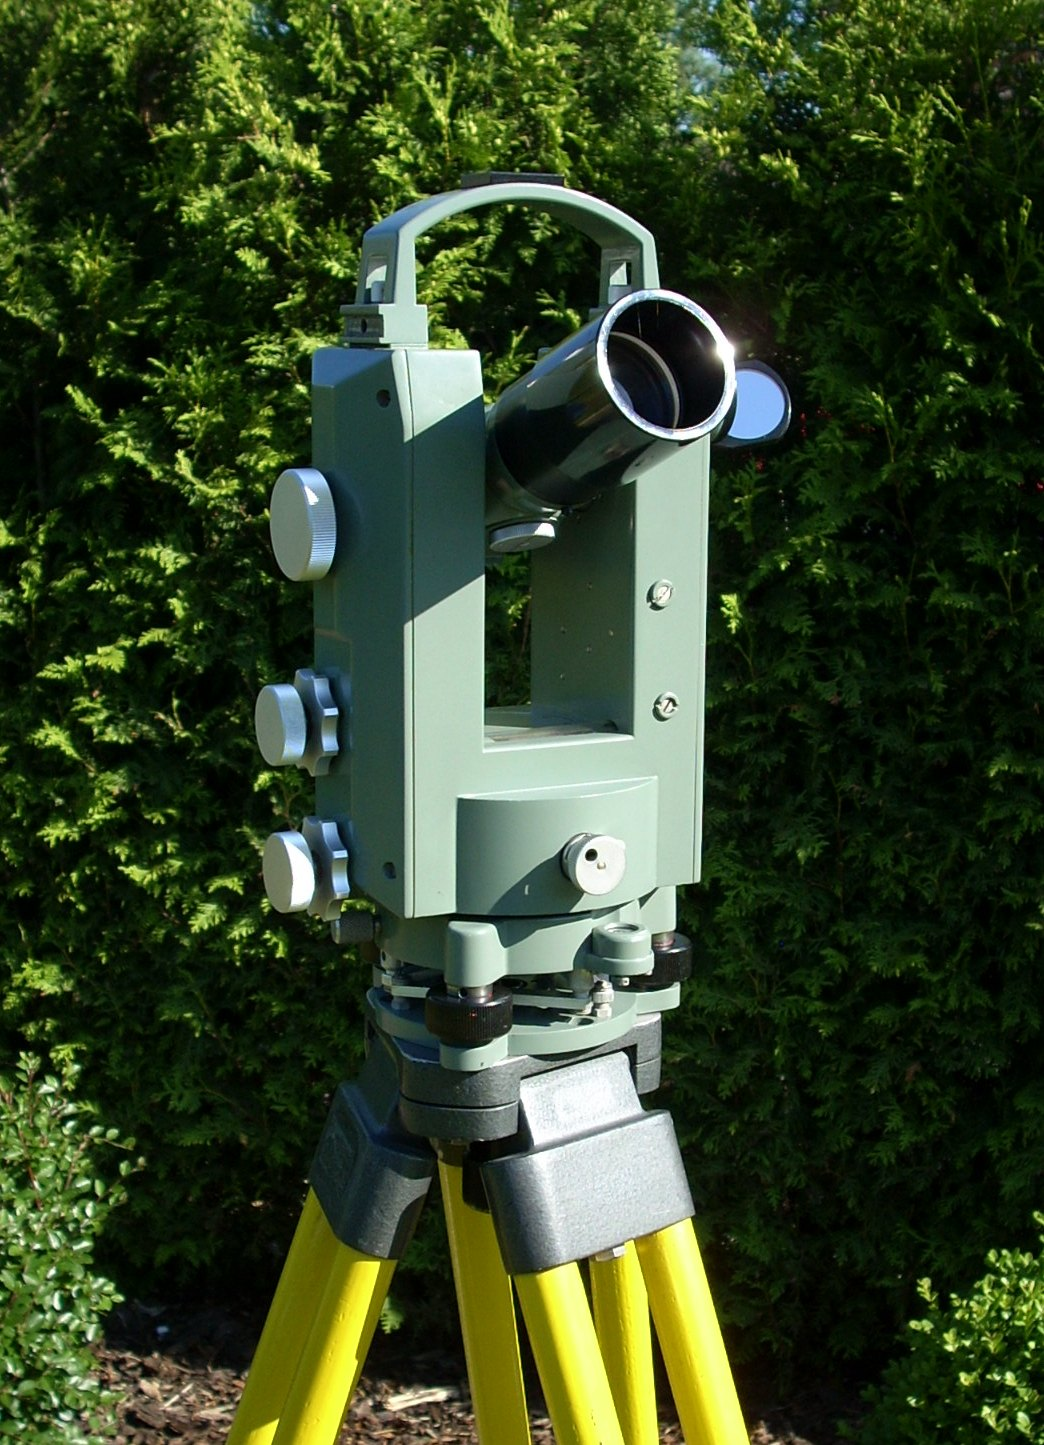
\includegraphics[width=0.3\textwidth]{Askania_Sekunden-Theodolit_TU_e_400.jpg}\quad
	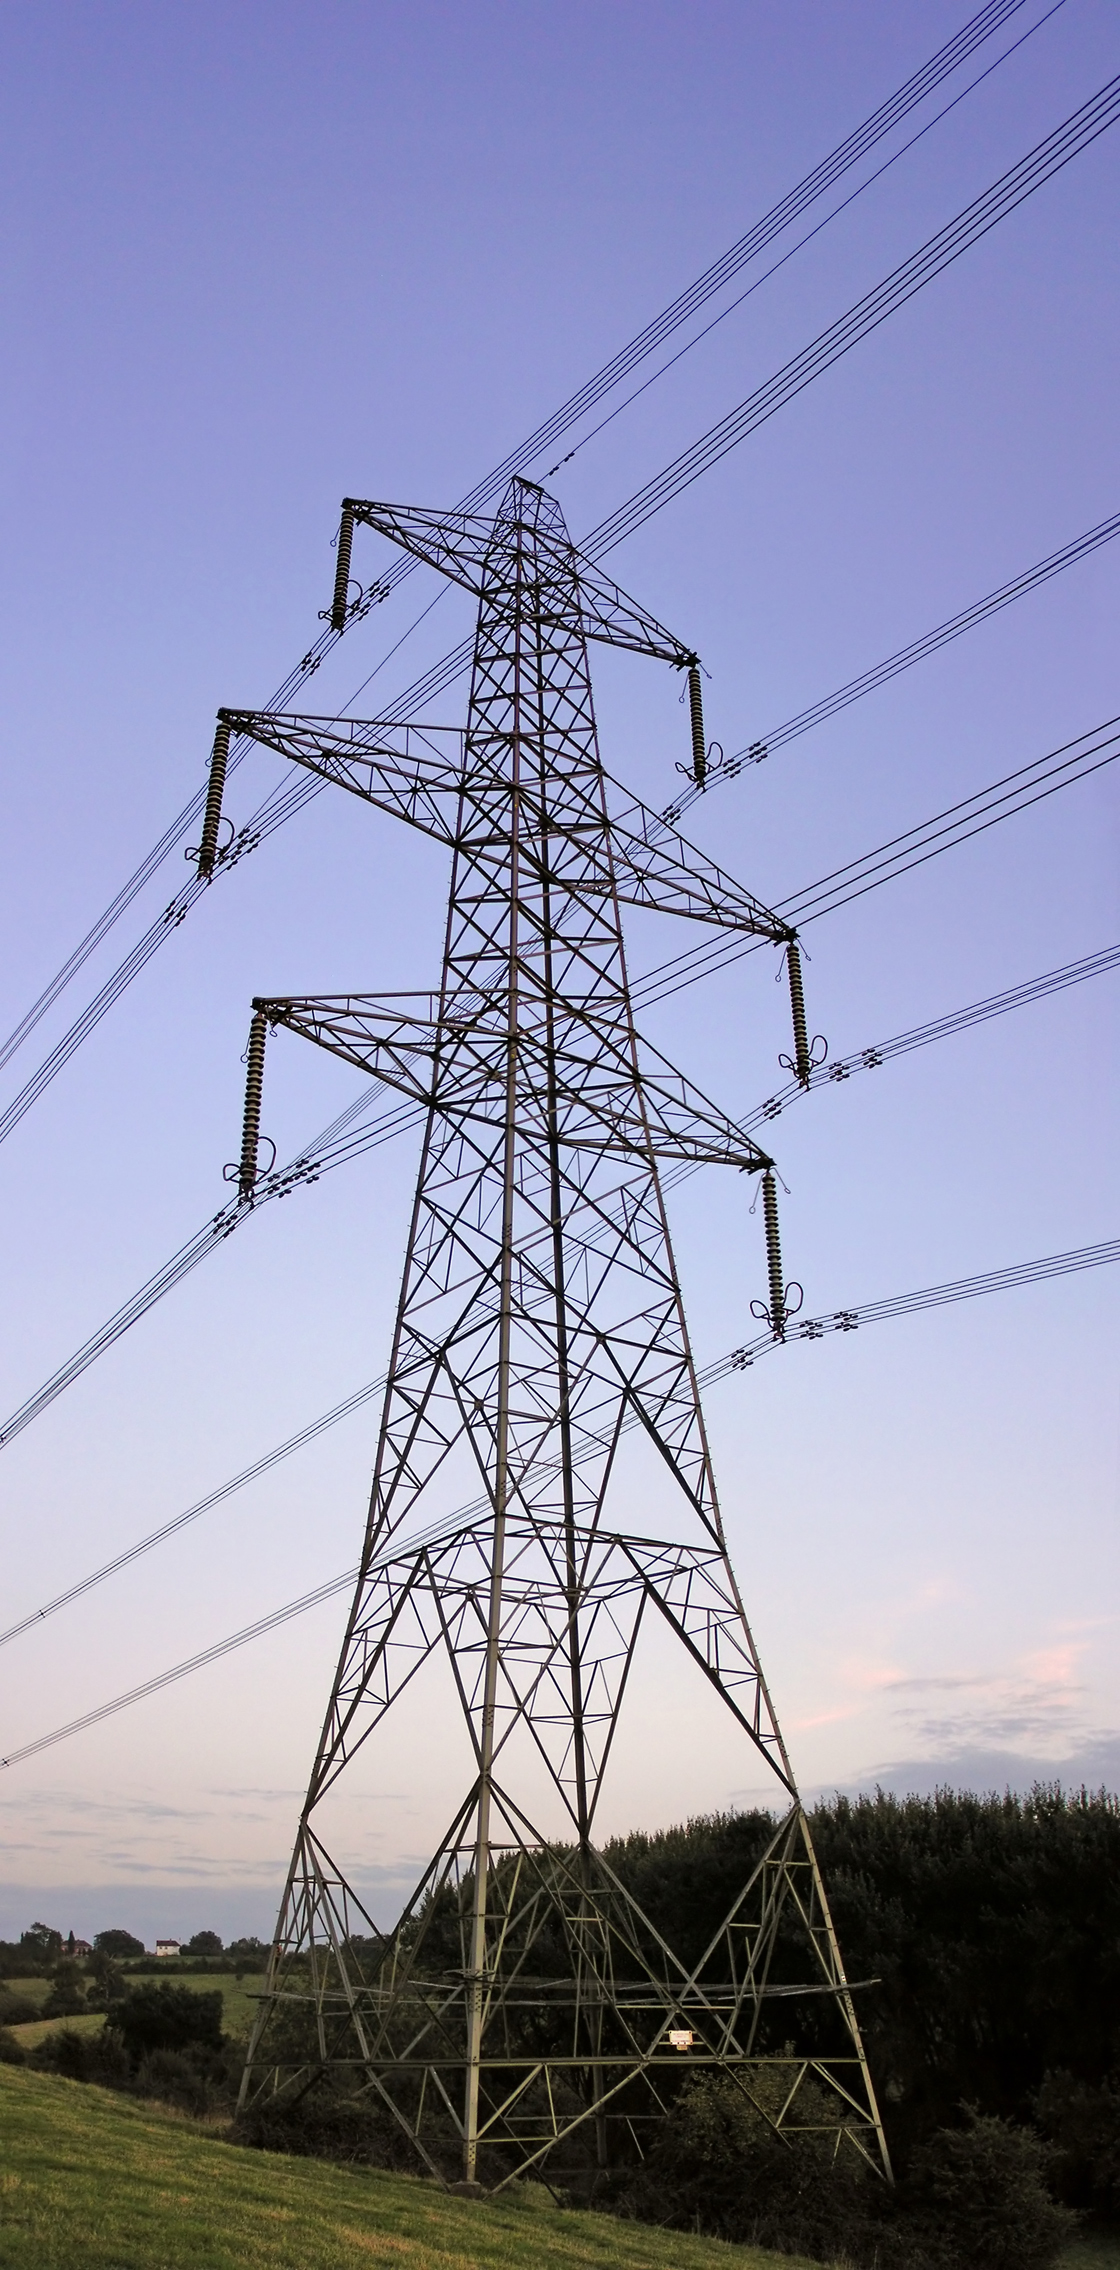
\includegraphics[width=0.3\textwidth]{Pylon_ds.jpg}
\end{image}
\end{center}


\subsection{Inleiding (Video, 1:27)}
\begin{expandable}
 \begin{center}
	 \youtube{2jGHOcxB8sI}
 \end{center}
\end{expandable}



\subsection{Inhoud}
\begin{expandable}
In deze module bestuderen we 
	\begin{itemize}
		\item het meten van hoeken in graden, minuten en seconden, maar in de wetenschap meestal in radialen.
        	\item de zogenaamde 'goniometrische getallen' van hoeken: sinus, cosinus en tangens
	    	\item een collectie eigenschappen en formules van hoeken en driehoeken: de Stelling van Pythagoras, cosinusregel, sinusregel etc.
        	\item de voorstelling op de goniometrische cirkel (met supplementaire, complementaire en tegengestelde hoeken)
	   	\item het oplossen van (al dan niet rechthoekige) driehoeken
	\end{itemize}

Het blijkt dat hoeken -misschien enigszins verrassend-  ook nauw verbonden zijn met de zogenaamde complexe getallen. Daarom besteden we in deze module ook daaraan aandacht. Complexe getallen worden ook gebruikt in andere delen van de wiskunde, zoals het oplossen van vergelijkingen, en in andere wetenschappen, bijvoorbeeld bij de studie van elektrische netwerken of trillingen.

We behandelen
	\begin{itemize}
		\item de definitie en voorstelling van complexe getallen, met de imaginaire eenheid i
		\item rekenen met complexe getallen en de complex toegevoegde $\bar{z}$ en norm $|z|$
		\item de exponentiële vorm $|z|e^{iθ}$ van complexe getallen
	\end{itemize}
\end{expandable}

\subsection{Wat moet je kennen en kunnen na deze module?}

\begin{expandable}
	\begin{itemize}
		\item Rekenen met hoeken in graden/minuten en seconden, en in radialen
		\item Je kent de sinus,cosinus en tangens van een hoek
		\item Je kent de hoofdformule van de goniometrie
	\end{itemize}
\end{expandable}

\subsection{Ken ik de leerstof al voldoende?}
\begin{expandable}
		  Druk uit in graden:
		  \begin{itemize}
	              \item 
			\begin{problem}
				\begin{hint} Een rechte hoek ... \end{hint}
				$\pi/2$: $\answer{90}^\circ$
			\end{problem}
	              \item 
			\begin{problem}
				\begin{hint} De helft van een rechte hoek ... \end{hint}
				$\pi/4$: $\answer{45}^\circ$
			\end{problem}
		      \item 
			\begin{problem}
				\begin{hint} $180^\circ = \pi$, dus $\dfrac{2\pi}{4} = ...$?\end{hint}
				$\dfrac{2\pi}{4}$: $\answer{120}^\circ$
			\end{problem}
		  \end{itemize}
\end{expandable}


\end{document}
